% ---------------------------------------------------------------------------
% Compilable LaTeX skeleton for the leakage-audit paper.
% It wires in the tables your pipeline already emits (tables/*.tex) and the
% figures (figures/*.pdf). Paste prose from ../DRAFT.md into the marked spots.
%
% BUILD (local):  pdflatex main  ->  bibtex main  ->  pdflatex main  ->  pdflatex main
% BUILD (Overleaf): just press Recompile (it runs the sequence for you).
%
% Paths below assume this file lives at  manuscript/latex/main.tex  and the repo
% tables/figures are two levels up. On Overleaf, either keep that folder layout
% or copy tables/ and figures/ next to main.tex and drop the ../../ prefixes.
% ---------------------------------------------------------------------------
\documentclass[11pt]{article}

\usepackage[margin=1in]{geometry}
\usepackage{booktabs}      % REQUIRED: the tables use \toprule/\midrule/\bottomrule
\usepackage{graphicx}      % for \includegraphics
\usepackage{amsmath}       % the table captions use $\pm$, $\to$
\usepackage[numbers,sort&compress]{natbib}  % citations; \citep / \citet
\usepackage{hyperref}
\usepackage{orcidlink}     % optional: the little ORCID icon (remove if unavailable)

\graphicspath{{../../figures/}}  % so \includegraphics{fig1_...} finds the PDFs

\title{Quantifying evaluation leakage in multi-species gene--disease link
prediction: a graded audit and a de-leaked benchmark}

\author{%
  Owen Liu\,\orcidlink{0009-0003-0476-5270}\thanks{Independent Researcher.} \and
  Ryan Tang\footnotemark[1] \and
  Daniel Augustine\footnotemark[1] \and
  [Mentor co-author]\thanks{[Affiliation].}
}
\date{}

\begin{document}
\maketitle

\begin{abstract}
% >>> Paste the Abstract from ../DRAFT.md here. <<<
Knowledge-graph embedding models predict gene--disease associations with high
reported scores that can be inflated by evaluation leakage. We present a graded
audit that separates and quantifies these mechanisms\ldots
\end{abstract}

\noindent\textbf{Keywords:} knowledge graph; knowledge graph embedding; link
prediction; gene--disease association; data leakage; benchmark evaluation; node
degree bias; reproducibility; Monarch Initiative; TransE; RotatE.

% ===========================================================================
\section{Introduction}
% >>> Paste Section 1 prose here. Example citation commands: <<<
Reported scores can be inflated by evaluation leakage
\citep{kapoor2023leakage, bernett2024guiding}. The phenomenon is established in
prior work, including on the Monarch graph itself
\citep{yilmaz2025bias, bradshaw2024effects, briere2025benchmarking}.

\section{Related work}
% >>> Paste Section 2 prose here. <<<

\section{Materials: the knowledge graph}
% >>> Paste Section 3 prose here. Then the table: <<<
\begin{table}[H]
\centering
\caption{Graph statistics for the Monarch-derived graph and the Hetionet robustness graph. The gene--disease target relation is GENE\_ASSOCIATED\_WITH\_CONDITION (Monarch) and DaG (Hetionet). Hetionet carries no cross-species orthology, so regime R3 is Monarch-only.}
\label{tab:graph_stats}
\begin{tabular}{lrr}
\toprule
Property & Monarch (this work) & Hetionet v1.0 (robustness) \\
\midrule
Nodes & 452,012 & 47,031 \\
Edges (directed) & 5,860,539 & 2,250,197 \\
Edges (unique undirected) & 5,583,381 & 2,107,709 \\
Node categories / metanodes & 8 & 11 \\
Relation / metaedge types & 28 & 24 \\
Degree mean & 25.9 & 99.7 \\
Degree median & 2 & 32 \\
Degree max & 20,662 & 23,879 \\
Gene nodes & 336,460 & 19,145 \\
Disease nodes & 14,339 & 136 \\
Gene--disease edges & 42,288 & 12,623 \\
Orthology edges & 510,703 & 0 (single-species) \\
\bottomrule
\end{tabular}
\end{table}
   % provides Table~\ref{tab:graph_stats}
As summarised in Table~\ref{tab:graph_stats}, the graph has 452{,}012 nodes.

\section{Methods}
% >>> Paste Section 4 prose here. <<<

\section{Results}
% >>> Paste Section 5 prose, interleaving the display items: <<<
\begin{table}[H]
\centering
\caption{Leakage audit on the held-out human gene--disease test edges (n = 4,228; mean $\pm$ SD over 3 seeds, 42/1/7). Columns 2--8 use the sampled protocol, 50 type-matched negatives per edge, which is what application papers report and which this audit treats as an inflated baseline rather than as a measure of model quality. The two right-hand columns give the same cells under filtered full ranking against the entire disease pool ($\approx$14,300 candidates); the full grid is S1 Table. The degree-preserving null (R2) is the only regime that materially reduces performance under either protocol, and it reduces it two to three times more under full ranking; redundancy (R1) and orthology (R3) are flat for the topological arm. AUROC for KGE is type-matched, comparable to the baselines' negatives. Statistics: 95\% bootstrap confidence intervals from 1,000 resamples over the per-edge reciprocal ranks; between-method and between-regime comparisons are two-sided paired bootstraps on aligned per-edge values; significance threshold $\alpha = 0.05$.}
\label{tab:audit}
\begin{tabular}{lrrrrrrrrr}
\toprule
Method & MRR R0 & MRR R1 & MRR R2 & MRR R3 & $\Delta$MRR R0$\to$R2 & AUROC R0 & Hits@10 R0 & Full-rank MRR R0 & Full-rank $\Delta$R0$\to$R2 \\
\midrule
Random & 0.091 $\pm$ 0.003 & 0.091 $\pm$ 0.003 & 0.091 $\pm$ 0.003 & 0.091 $\pm$ 0.003 & +0\% & 0.503 $\pm$ 0.001 & 0.199 $\pm$ 0.002 & 0.001 & +0\% \\
Common-Neighbors & 0.441 $\pm$ 0.001 & 0.442 $\pm$ 0.001 & 0.247 $\pm$ 0.001 & 0.443 $\pm$ 0.002 & -44\% & 0.736 $\pm$ 0.000 & 0.522 $\pm$ 0.001 & 0.118 & -88\% \\
Adamic-Adar & 0.459 $\pm$ 0.000 & 0.459 $\pm$ 0.002 & 0.262 $\pm$ 0.000 & 0.460 $\pm$ 0.003 & -43\% & 0.738 $\pm$ 0.000 & 0.528 $\pm$ 0.001 & 0.133 & -89\% \\
Jaccard & 0.397 $\pm$ 0.001 & 0.398 $\pm$ 0.002 & 0.201 $\pm$ 0.001 & 0.399 $\pm$ 0.001 & -49\% & 0.690 $\pm$ 0.001 & 0.474 $\pm$ 0.002 & 0.106 & -91\% \\
Preferential-Attachment & 0.587 $\pm$ 0.002 & 0.582 $\pm$ 0.001 & 0.589 $\pm$ 0.002 & 0.581 $\pm$ 0.002 & +0\% & 0.794 $\pm$ 0.000 & 0.774 $\pm$ 0.001 & 0.025 & +1\% \\
TransE & 0.799 $\pm$ 0.000 & 0.750 $\pm$ 0.004 & 0.611 $\pm$ 0.004 & 0.800 $\pm$ 0.002 & -24\% & 0.962 $\pm$ 0.001 & 0.975 $\pm$ 0.001 & 0.079 & -71\% \\
RotatE & 0.827 $\pm$ 0.007 & 0.757 $\pm$ 0.004 & 0.655 $\pm$ 0.004 & 0.830 $\pm$ 0.004 & -21\% & 0.967 $\pm$ 0.001 & 0.974 $\pm$ 0.000 & 0.108 & -70\% \\
DistMult & 0.669 $\pm$ 0.007 & 0.591 $\pm$ 0.010 & 0.426 $\pm$ 0.005 & 0.689 $\pm$ 0.006 & -36\% & 0.937 $\pm$ 0.002 & 0.934 $\pm$ 0.004 & 0.050 & -78\% \\
ComplEx & 0.685 $\pm$ 0.004 & 0.594 $\pm$ 0.003 & 0.431 $\pm$ 0.027 & 0.692 $\pm$ 0.007 & -37\% & 0.918 $\pm$ 0.004 & 0.913 $\pm$ 0.007 & 0.055 & -82\% \\
\bottomrule
\end{tabular}
\end{table}

\noindent\footnotesize Paired-bootstrap MRR difference (Adamic-Adar $-$ method; R0, seed 42, 1,000 resamples, n=4,228): Common-Neighbors $\Delta$=+0.017 (p$<$0.001); Jaccard $\Delta$=+0.060 (p$<$0.001); Preferential-Attachment $\Delta$=-0.130 (p$<$0.001); Random $\Delta$=+0.365 (p$<$0.001). All significant at p$<$0.001 (two-sided).\normalsize

          % Table~\ref{tab:audit}
The degree-preserving null is the only regime that materially reduces
performance (Table~\ref{tab:audit}).

\begin{figure}[t]
  \centering
  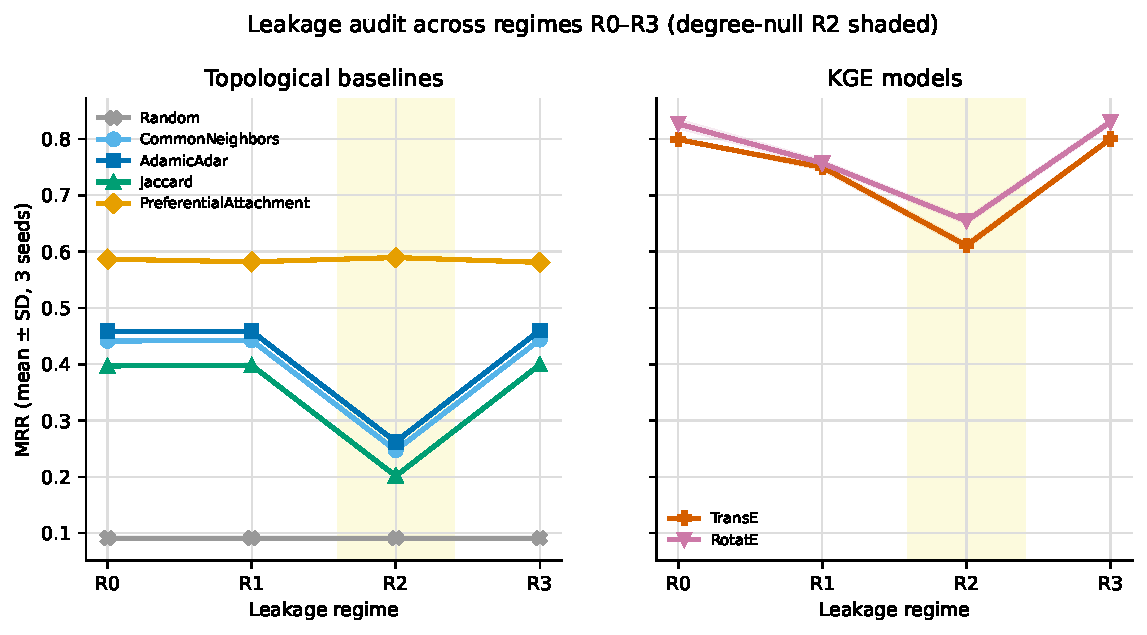
\includegraphics[width=\linewidth]{fig2_leakage_audit.pdf}
  \caption{Leakage audit across regimes.}
  \label{fig:audit}
\end{figure}

\begin{table}[H]
\centering
\caption{Degree-null decomposition of R0 ranking performance (200 degree-preserving, type-preserving permutation replicates; R0 evaluation held fixed). The structure column is the residual above what pure node degree explains; the permutation p-value is the add-one empirical estimator $(b+1)/(B+1)$, where $b$ is the number of null replicates with MRR $\geq$ the real R0 MRR. With 200 replicates the add-one estimator is bounded below by $1/(200+1)\approx0.005$, so structural methods (every null replicate below the real MRR) sit at this floor; their residuals nonetheless exceed the null mean by $>$50 null standard deviations. Degree sequence preserved: True. Preferential-Attachment sanity: real 0.589 vs null 0.591 (unchanged $\to$ the null preserves the degree sequence). The permutation test is the coarser of the two instruments reported; the primary significance test for the R0$\to$R2 drop is a two-sided paired bootstrap over the 4,228 aligned per-edge reciprocal ranks. Statistics: 95\% bootstrap confidence intervals from 1,000 resamples over the per-edge reciprocal ranks; between-method and between-regime comparisons are two-sided paired bootstraps on aligned per-edge values; significance threshold $\alpha = 0.05$.}
\label{tab:degree_null}
\begin{tabular}{lrrrrr}
\toprule
Method & Real R0 MRR & Degree-null MRR & Structure (real$-$null) & Perm. p & Structure > degree? \\
\midrule
Common-Neighbors & 0.441 & 0.248 $\pm$ 0.003 & +0.193 & 0.005 & yes \\
Adamic-Adar & 0.458 & 0.262 $\pm$ 0.004 & +0.196 & 0.005 & yes \\
Jaccard & 0.398 & 0.202 $\pm$ 0.003 & +0.196 & 0.005 & yes \\
Preferential-Attachment & 0.589 & 0.591 $\pm$ 0.000 & -0.002 & 1.000 & no \\
Random & 0.094 & 0.094 $\pm$ 0.000 & -0.000 & 1.000 & no \\
\bottomrule
\end{tabular}
\end{table}
    % degree decomposition
\begin{table}[t]
\centering
\caption{Cross-graph robustness: the same audit rerun unmodified on Hetionet (DaG task; mean $\pm$ SD over 3 seeds). Hetionet has no cross-species orthology, so R3 is omitted. The R0$\to$R2 degree-null drop reproduces the Monarch pattern on an independent graph.}
\label{tab:hetionet}
\begin{tabular}{lrrrr}
\toprule
Method & MRR R0 & MRR R1 & MRR R2 & $\Delta$MRR R0$\to$R2 \\
\midrule
Random & 0.092 $\pm$ 0.001 & 0.092 $\pm$ 0.001 & 0.092 $\pm$ 0.001 & +0\% \\
CommonNeighbors & 0.269 $\pm$ 0.003 & 0.268 $\pm$ 0.002 & 0.173 $\pm$ 0.001 & -35\% \\
AdamicAdar & 0.285 $\pm$ 0.005 & 0.284 $\pm$ 0.004 & 0.178 $\pm$ 0.002 & -37\% \\
Jaccard & 0.162 $\pm$ 0.002 & 0.162 $\pm$ 0.001 & 0.104 $\pm$ 0.001 & -36\% \\
PreferentialAttachment & 0.231 $\pm$ 0.002 & 0.231 $\pm$ 0.002 & 0.231 $\pm$ 0.002 & -0\% \\
\bottomrule
\end{tabular}
\end{table}
       % Hetionet replication
\begin{table}[H]
\centering
\caption{Full-ranking robustness of the leakage regimes. Each held-out human gene--disease test edge has its true disease ranked against the entire type-matched disease pool (size $D$ per regime), excluding the gene's known training and test tails (filtered) -- the strictest protocol available, and stricter than the 50 sampled negatives of Table~\ref{tab:audit}. \textbf{Panel A} is the knowledge-graph embedding arm (mean $\pm$ SD over 3 seeds, 1, 7, 42); \textbf{Panel B} is the topological arm. $\Delta$MRR vs R0 is the per-method change from the standard regime. Absolute MRR is far lower than under sampled negatives (the true disease competes with $\sim$14k pool diseases rather than 50), but the \emph{ordering} of the regime effects is preserved throughout: the R2 degree-preserving null causes by far the largest drop in both arms, while R3 (orthology-blocked) lowers no method's score in either -- the same pattern as the sampled-negative audit -- so the regime effects are not artifacts of negative sampling. Panel A $\Delta$MRR vs R0: R1 -32\% (ComplEx), -22\% (DistMult), -19\% (RotatE), -10\% (TransE); R2 -82\% (ComplEx), -78\% (DistMult), -70\% (RotatE), -71\% (TransE); R3 +8\% (ComplEx), +16\% (DistMult), +3\% (RotatE), +2\% (TransE). R2 costs every embedding model 70-82\% of its MRR, and R1 (redundancy) is the regime that separates the two arms: it costs the KGE models 10-32\% of MRR against only 2\% for the overlap heuristics, which is the arm-specific redundancy leak of the sampled-negative audit reappearing at larger magnitude under the stricter protocol. R3 lowers no model's MRR under this protocol either, but the size of the gain is not uniform: the translational pair stays within +3\% while the bilinear pair rises 8-16\%, so blocking the cross-species bridges is mildly helpful to the bilinear models rather than merely uninformative -- a stronger refutation of the orthology-leak hypothesis than a flat null, and in the opposite direction from leakage. Panel B is a single deterministic run per regime (the topological scorers carry no seed; the Random control is the analytic chance floor), so no SD is reported, and AUROC is not defined for the ranking-only protocol. n=4,228 test edges; ranks were verified against a brute-force loop of the same scorers over the full pool on 150 sampled edges per regime (exact agreement). Under full ranking the R0$\to$R2 collapse of the overlap heuristics deepens to 88-91\% (it is 43-49\% under 50 sampled negatives), while Preferential-Attachment moves by +1\%: the degree-only control is unmoved by the degree-preserving null under the strictest protocol, so the sampled-negative effect sizes are lower bounds. 30 cold-start test genes (absent from the training vocabulary) receive the worst possible rank. Statistics: 95\% bootstrap confidence intervals from 1,000 resamples over the per-edge reciprocal ranks; between-method and between-regime comparisons are two-sided paired bootstraps on aligned per-edge values; significance threshold $\alpha = 0.05$.}
\label{tab:fullrank_robustness}
\begin{tabular}{lrrrrrrrr}
\toprule
Model & Regime & Pool D & MRR & Hits@1 & Hits@3 & Hits@10 & AUROC (type) & $\Delta$MRR vs R0 \\
\midrule
\multicolumn{9}{l}{\textit{Panel A. Knowledge-graph embedding}} \\
TransE & R0 standard & 14,307 & 0.079 $\pm$ 0.001 & 0.036 $\pm$ 0.001 & 0.072 $\pm$ 0.002 & 0.150 $\pm$ 0.003 & 0.962 $\pm$ 0.002 & ref \\
TransE & R1 redundancy & 14,252 & 0.071 $\pm$ 0.003 & 0.031 $\pm$ 0.002 & 0.066 $\pm$ 0.002 & 0.138 $\pm$ 0.008 & 0.954 $\pm$ 0.001 & -10\% \\
TransE & R2 degree-null & 14,307 & 0.023 $\pm$ 0.002 & 0.005 $\pm$ 0.001 & 0.014 $\pm$ 0.003 & 0.042 $\pm$ 0.004 & 0.879 $\pm$ 0.001 & -71\% \\
TransE & R3 orthology-blocked & 14,137 & 0.080 $\pm$ 0.004 & 0.034 $\pm$ 0.003 & 0.077 $\pm$ 0.005 & 0.155 $\pm$ 0.008 & 0.963 $\pm$ 0.000 & +2\% \\
RotatE & R0 standard & 14,307 & 0.108 $\pm$ 0.004 & 0.053 $\pm$ 0.002 & 0.107 $\pm$ 0.003 & 0.202 $\pm$ 0.003 & 0.967 $\pm$ 0.001 & ref \\
RotatE & R1 redundancy & 14,252 & 0.088 $\pm$ 0.002 & 0.037 $\pm$ 0.002 & 0.086 $\pm$ 0.002 & 0.178 $\pm$ 0.002 & 0.955 $\pm$ 0.001 & -19\% \\
RotatE & R2 degree-null & 14,307 & 0.032 $\pm$ 0.002 & 0.006 $\pm$ 0.001 & 0.021 $\pm$ 0.001 & 0.067 $\pm$ 0.007 & 0.889 $\pm$ 0.000 & -70\% \\
RotatE & R3 orthology-blocked & 14,137 & 0.111 $\pm$ 0.003 & 0.055 $\pm$ 0.003 & 0.110 $\pm$ 0.003 & 0.211 $\pm$ 0.004 & 0.969 $\pm$ 0.001 & +3\% \\
DistMult & R0 standard & 14,307 & 0.050 $\pm$ 0.003 & 0.020 $\pm$ 0.002 & 0.045 $\pm$ 0.004 & 0.098 $\pm$ 0.005 & 0.937 $\pm$ 0.002 & ref \\
DistMult & R1 redundancy & 14,252 & 0.039 $\pm$ 0.002 & 0.014 $\pm$ 0.002 & 0.032 $\pm$ 0.004 & 0.076 $\pm$ 0.006 & 0.897 $\pm$ 0.002 & -22\% \\
DistMult & R2 degree-null & 14,307 & 0.011 $\pm$ 0.001 & 0.001 $\pm$ 0.001 & 0.006 $\pm$ 0.001 & 0.020 $\pm$ 0.002 & 0.832 $\pm$ 0.002 & -78\% \\
DistMult & R3 orthology-blocked & 14,137 & 0.058 $\pm$ 0.003 & 0.026 $\pm$ 0.003 & 0.050 $\pm$ 0.003 & 0.108 $\pm$ 0.002 & 0.943 $\pm$ 0.001 & +16\% \\
ComplEx & R0 standard & 14,307 & 0.055 $\pm$ 0.006 & 0.020 $\pm$ 0.005 & 0.046 $\pm$ 0.008 & 0.114 $\pm$ 0.008 & 0.918 $\pm$ 0.004 & ref \\
ComplEx & R1 redundancy & 14,252 & 0.037 $\pm$ 0.002 & 0.012 $\pm$ 0.001 & 0.028 $\pm$ 0.001 & 0.072 $\pm$ 0.005 & 0.891 $\pm$ 0.004 & -32\% \\
ComplEx & R2 degree-null & 14,307 & 0.010 $\pm$ 0.001 & 0.001 $\pm$ 0.000 & 0.004 $\pm$ 0.000 & 0.017 $\pm$ 0.003 & 0.799 $\pm$ 0.006 & -82\% \\
ComplEx & R3 orthology-blocked & 14,137 & 0.059 $\pm$ 0.006 & 0.022 $\pm$ 0.004 & 0.052 $\pm$ 0.006 & 0.118 $\pm$ 0.014 & 0.917 $\pm$ 0.009 & +8\% \\
\multicolumn{9}{l}{\textit{Panel B. Topological baselines}} \\
Random & R0 standard & 14,307 & 0.001 & 0.000 & 0.000 & 0.001 & -- & ref \\
Random & R1 redundancy & 14,252 & 0.001 & 0.000 & 0.000 & 0.001 & -- & +0\% \\
Random & R2 degree-null & 14,307 & 0.001 & 0.000 & 0.000 & 0.001 & -- & +0\% \\
Random & R3 orthology-blocked & 14,137 & 0.001 & 0.000 & 0.000 & 0.001 & -- & +1\% \\
Common-Neighbors & R0 standard & 14,307 & 0.118 & 0.076 & 0.125 & 0.192 & -- & ref \\
Common-Neighbors & R1 redundancy & 14,252 & 0.116 & 0.074 & 0.123 & 0.191 & -- & -2\% \\
Common-Neighbors & R2 degree-null & 14,307 & 0.014 & 0.001 & 0.007 & 0.049 & -- & -88\% \\
Common-Neighbors & R3 orthology-blocked & 14,137 & 0.117 & 0.075 & 0.123 & 0.191 & -- & -1\% \\
Adamic-Adar & R0 standard & 14,307 & 0.133 & 0.091 & 0.143 & 0.214 & -- & ref \\
Adamic-Adar & R1 redundancy & 14,252 & 0.130 & 0.088 & 0.140 & 0.211 & -- & -2\% \\
Adamic-Adar & R2 degree-null & 14,307 & 0.014 & 0.000 & 0.008 & 0.048 & -- & -89\% \\
Adamic-Adar & R3 orthology-blocked & 14,137 & 0.132 & 0.090 & 0.143 & 0.213 & -- & -1\% \\
Jaccard & R0 standard & 14,307 & 0.106 & 0.079 & 0.113 & 0.150 & -- & ref \\
Jaccard & R1 redundancy & 14,252 & 0.104 & 0.077 & 0.112 & 0.150 & -- & -2\% \\
Jaccard & R2 degree-null & 14,307 & 0.009 & 0.003 & 0.005 & 0.020 & -- & -91\% \\
Jaccard & R3 orthology-blocked & 14,137 & 0.106 & 0.079 & 0.113 & 0.151 & -- & -0\% \\
Preferential-Attachment & R0 standard & 14,307 & 0.025 & 0.000 & 0.000 & 0.081 & -- & ref \\
Preferential-Attachment & R1 redundancy & 14,252 & 0.025 & 0.000 & 0.000 & 0.081 & -- & -0\% \\
Preferential-Attachment & R2 degree-null & 14,307 & 0.025 & 0.000 & 0.000 & 0.081 & -- & +1\% \\
Preferential-Attachment & R3 orthology-blocked & 14,137 & 0.025 & 0.000 & 0.000 & 0.080 & -- & -1\% \\
\bottomrule
\end{tabular}
\end{table}
  % full-ranking robustness

\begin{figure}[t]
  \centering
  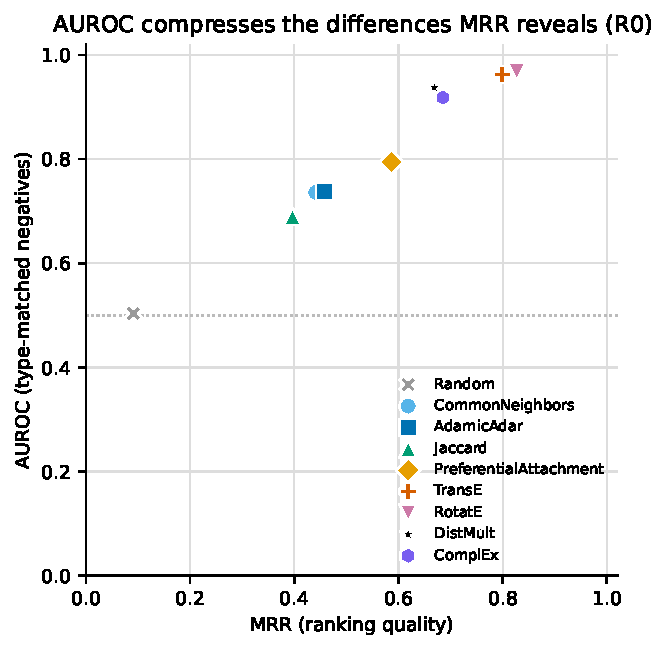
\includegraphics[width=\linewidth]{fig1_auroc_mrr_dissociation.pdf}
  \caption{AUROC stays high while MRR collapses under the degree null.}
  \label{fig:dissociation}
\end{figure}

\section{Discussion}
% >>> Paste Section 6 prose here. <<<

\section{Conclusion}
% >>> Paste Section 7 prose here. <<<

\section*{Data and code availability}
Archived at Zenodo (DOI \texttt{10.5281/zenodo.21398832}) and on GitHub.

\section*{Author contributions}
% >>> Paste from ../DRAFT.md. <<<

\section*{Competing interests}
The authors declare no competing interests.

% ===========================================================================
\bibliographystyle{plainnat}   % author-year: use plainnat; numbered: unsrtnat
\bibliography{references}       % reads references.bib
\end{document}
